\documentclass[10pt,conference,a4paper]{IEEEtran}
\usepackage[T1]{fontenc}
\usepackage[utf8]{inputenc}
\usepackage{amsmath,amssymb}
\usepackage{booktabs,array}
\usepackage{graphicx}
\usepackage{enumitem}
\usepackage{xcolor}
\usepackage{microtype}
\usepackage{fancyhdr}
\usepackage{lastpage}
\definecolor{sphereblue}{RGB}{15,64,96}
\setlength{\parindent}{1em}
\setlength{\parskip}{1.2pt}
\linespread{1.01}
\setlength{\columnsep}{0.22in}
\setlist{topsep=2pt,partopsep=0pt,itemsep=1pt,parsep=0pt}
\pagestyle{fancy}
\fancyhf{}
\fancyhead[L]{\scriptsize SPACESUIT THERMAL SHIELDING KIT}
\fancyhead[R]{\scriptsize Team Engineering Report}
\fancyfoot[C]{\scriptsize \thepage\ / \pageref{LastPage}}
\renewcommand{\headrulewidth}{0.3pt}
\renewcommand{\footrulewidth}{0pt}
\title{SPACESUIT THERMAL SHIELDING KIT\\\large Team Engineering Report for the SPHERE Initiative}
\author{Piyath Vithanage, Elio Krollpfeiffer, Dilan Fernando, and Nuhansee Migelhewage\\
Professorship of Human Spaceflight Technology\\Prof. Dr.-Ing. Gisela Detrell\\
TUM School of Engineering and Design, Technical University of Munich}
\begin{document}
\maketitle
\begin{abstract}
The SPHERE team designed a classroom experiment that compares four insulation arrangements around a 100 mL warm-water core. Students record 16 temperatures, generate a Newtonian cooling reference curve, and evaluate the difference between measurement and prediction. The worked test ranked the full cotton--bubble-wrap--Mylar package first for heat retention. The report also explains why the water-bath test is not a vacuum or spacesuit qualification test.
\end{abstract}
\begin{IEEEkeywords}
heat transfer, Newtonian cooling, insulation, classroom experiment, data logging, model validation
\end{IEEEkeywords}


\section*{Executive Summary and Project Definition}

This report presents the project's SPACESUIT THERMAL SHIELDING KIT. The project was built the project around one engineering question: how much does a chosen layer arrangement reduce the cooling rate of the same 100 mL water-filled core under the same cold-water boundary? The kit combines four physical test articles, a browser-based Mission Control page, manual temperature logging, and a Newtonian cooling model. The project aim was to make heat transfer measurable in one school lesson without requiring specialist data-acquisition hardware.

The four conditions are a bare control, two layers of bubble wrap, a Mylar-only wrap, and a full multilayer package made from cotton, bubble wrap, and Mylar. Students record the core temperature once per minute from 0 to 15 minutes. The website plots the recorded values against a reference curve and calculates residuals and mean absolute error. In the worked data, the full multilayer package retained the most heat. Mylar alone performed poorly in the water-bath setup, which showed why a reflective material cannot be judged without considering contact, convection, wetting, gaps, and closure quality.

\subsection*{Main outcome}

The team produced a reusable experiment that links construction, measurement, modelling, and evaluation. The activity does not reproduce vacuum and does not test materials for real spacesuit use. It is a controlled teaching model for comparing cooling behaviour. The final design uses identical glass jars, a target start temperature near 80 $^\circ$C, a measured ice-water bath, a centred probe, and a 16-point temperature record.

\begin{center}\footnotesize
\setlength{\tabcolsep}{2.5pt}
\renewcommand{\arraystretch}{1.14}
\begin{tabular}{>{\raggedright\arraybackslash}p{0.31\columnwidth}>{\raggedright\arraybackslash}p{0.61\columnwidth}}
\toprule
\textbf{Item} & \textbf{Final project setting} \\
\midrule
Thermal core & 100 mL water in matched glass jars \\
Boundary & Measured ice-water bath \\
Sampling & Every minute from 0 to 15 min \\
Outputs & Measured curve, model curve, residuals, MAE \\
Lesson length & About 55-70 min including setup and review \\
\bottomrule
\end{tabular}
\end{center}

\subsection*{Project scope}

The team developed the thermal model, experimental method, physical test articles, browser application, telemetry workflow, assessment activities, classroom documentation, safety guidance, and final learning resources as one integrated engineering package.

\section*{1 Project Context and Requirements}

\subsection*{1.1 Context}

SPHERE uses human-spaceflight engineering as the setting for classroom activities. Thermal protection was selected because students can see the construction, measure a temperature change, and compare a real curve with a mathematical prediction. The spacesuit story gives the task a clear purpose, but the measured system is a jar in a water bath. This distinction remains visible throughout the manuals and website.

\subsection*{1.2 Engineering requirements}

\begin{itemize}[leftmargin=*,nosep]

\item Produce a visible difference between configurations within a 15-minute test.

\item Use parts that a school can replace locally.

\item Keep the procedure understandable without prior differential-equation study.

\item Run on ordinary laptops and tablets without accounts, pairing, or a native app.

\item Keep hot water, cold bath water, and electronic displays separated.

\item Use the same variables and test settings in the website, manuals, worksheet, and report.

\end{itemize}

\subsection*{1.3 Learning requirements}

Students should be able to distinguish conduction, convection, and radiation; explain the meaning of an effective cooling constant; collect an ordered time series; compare measurement with prediction; and discuss uncertainty. The design also aimed them to see that an unexpected result is useful evidence. A disagreement should lead to checks of the setup and assumptions, not to editing the data until it matches the model.

\begin{center}\footnotesize
\setlength{\tabcolsep}{2.5pt}
\renewcommand{\arraystretch}{1.14}
\begin{tabular}{>{\raggedright\arraybackslash}p{0.25\columnwidth}>{\raggedright\arraybackslash}p{0.31\columnwidth}>{\raggedright\arraybackslash}p{0.34\columnwidth}}
\toprule
\textbf{Requirement} & \textbf{Design response} & \textbf{Check} \\
\midrule
Comparable cores & Matched 100 mL jars & Same geometry and fill \\
Repeatable boundary & Shared ice-water bath & Measure bath temperature \\
Safe handling & Adult pours hot water & Pre-run safety checklist \\
Accessible software & Static browser app & No login or driver \\
Traceable result & 16 raw readings retained & Table and graph agree \\
\bottomrule
\end{tabular}
\end{center}

\subsection*{1.4 Decisions made during development}

The team first considered automatic sensors and wireless transfer. That option was rejected because it would shift attention from the thermal problem to pairing, drivers, and battery faults. Manual entry makes the observation step explicit and is easier for a teacher to recover when something goes wrong. The design question was also changed from a general spacesuit demonstration to a controlled comparison of cooling rate. This change produced measurable inputs, a fair-test procedure, and a result that students could defend.

\section*{2 Thermodynamic Model}

\subsection*{2.1 Lumped cooling model}

The model treats the water as one thermal mass with a uniform temperature. This is an approximation, but it gives a useful reference for a short classroom test. The stored sensible energy change is

\begin{equation}Q = m c_p \Delta T.\end{equation}

For 100 mL of water, the mass is approximately 0.10 kg. With a water heat capacity of about 4184 J kg$^{-1}$ K$^{-1}$, a 10 K drop represents about 4.18 kJ leaving the water. The jar, probe, and insulation also store energy, so this value is an estimate rather than a complete energy balance.

For a body losing heat to an environment at approximately constant temperature, the team use

\begin{equation}m c_p \frac{dT}{dt} = -hA(T-T_{env}),\end{equation}

which gives the reference curve

\begin{equation}T(t)=T_{env}+(T_0-T_{env})e^{-kt}.\end{equation}

The website uses minutes, so the effective cooling constant k is in min$^{-1}$. It combines geometry, boundary conditions, thermal mass, and all heat-loss paths. It is not the material conductivity of cotton, bubble wrap, or Mylar.

\subsection*{2.2 Model coefficients}

\begin{center}\footnotesize
\setlength{\tabcolsep}{2.5pt}
\renewcommand{\arraystretch}{1.14}
\begin{tabular}{>{\raggedright\arraybackslash}p{0.25\columnwidth}>{\raggedright\arraybackslash}p{0.31\columnwidth}>{\raggedright\arraybackslash}p{0.34\columnwidth}}
\toprule
\textbf{Condition} & \textbf{Reference k (min\textasciicircum{}-1)} & \textbf{Model T15 for 80/0 $^\circ$C} \\
\midrule
Bare control & 0.150 & 8.4 $^\circ$C \\
Bubble wrap & 0.040 & 43.9 $^\circ$C \\
Mylar only & 0.121 & 13.0 $^\circ$C \\
Full MLI & 0.015 & 63.9 $^\circ$C \\
\bottomrule
\end{tabular}
\end{center}

\subsection*{2.3 Interpretation}

Cotton and bubble wrap reduce direct solid contact and trap low-density regions. Mylar mainly changes radiative exchange when a suitable air gap exists. In a water bath, conduction and convection can dominate, especially if water touches the wrap or enters through the neck. This is why the Mylar-only condition should not be treated as a direct test of spacecraft multilayer insulation.

For runs with different starting temperatures, the team compare the dimensionless temperature above the boundary:

\begin{equation}\theta(t)=\frac{T(t)-T_{env}}{T_0-T_{env}}.\end{equation}

\section*{3 Hardware and Test Configurations}

\subsection*{3.1 Apparatus}

The physical system uses four matched 100 mL glass jars, four digital probe thermometers, a separate bath thermometer, one stable bucket or deep container, insulation materials, a timer, towels, and heat-resistant handling tools. Each probe is suspended near the centre of the water volume. The display and cable connector stay dry and outside the bath.

\begin{center}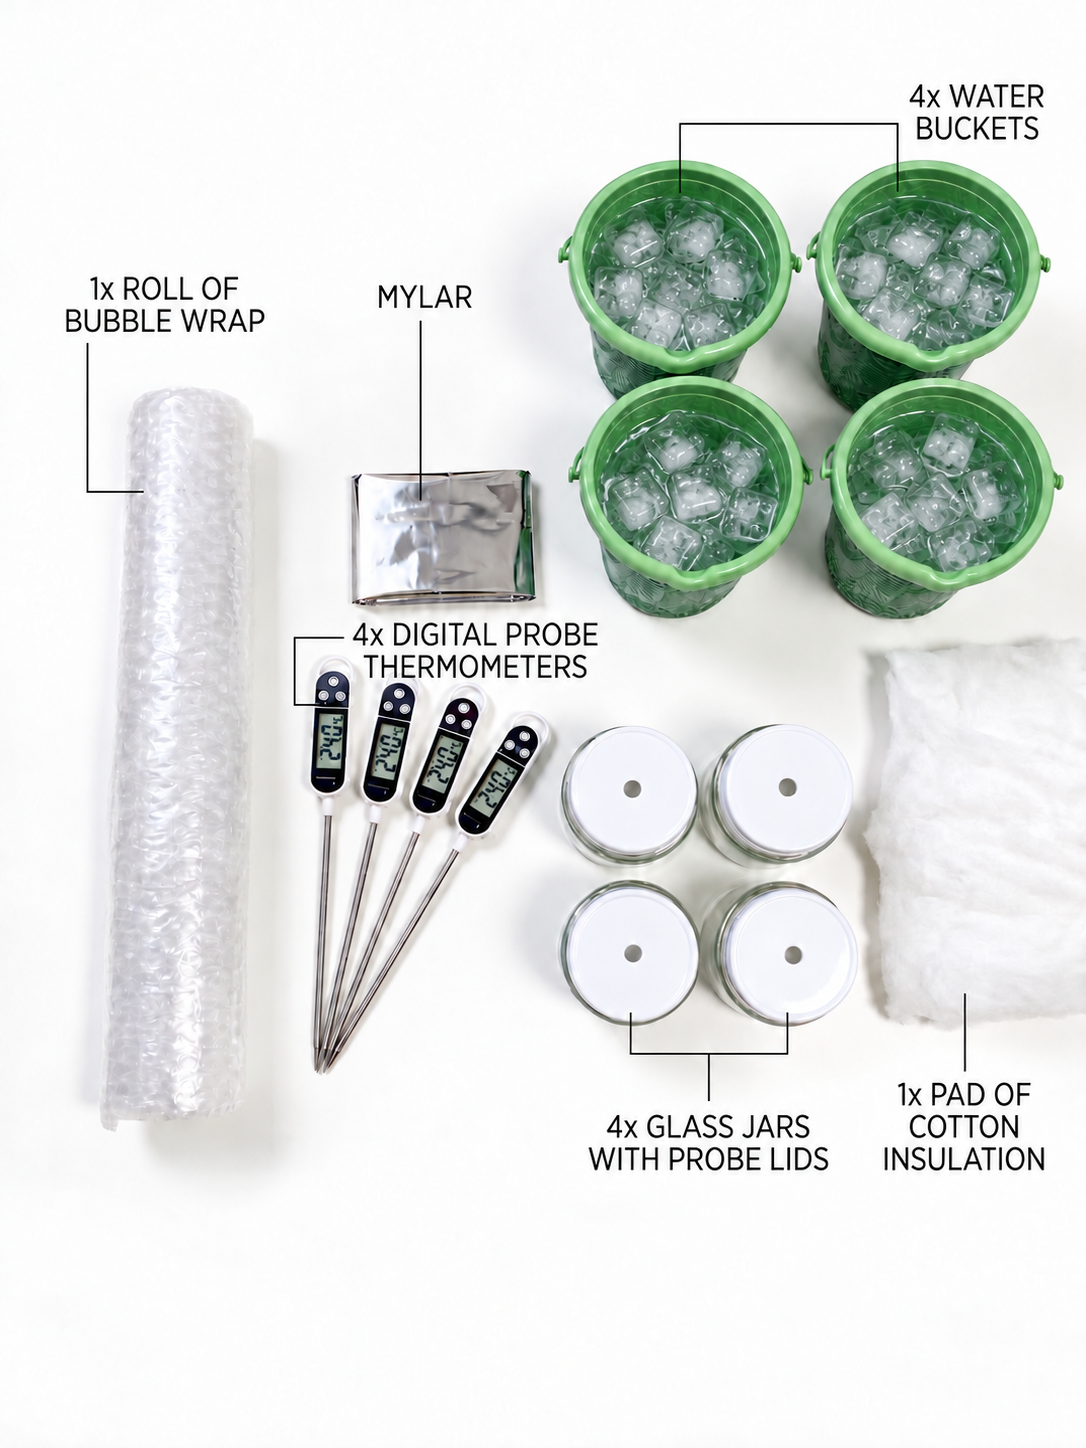
\includegraphics[width=0.78\linewidth]{assets/equipments.png}\par\vspace{2pt}{\footnotesize Image A. Complete apparatus set used for the four-condition classroom experiment.}\end{center}

\begin{center}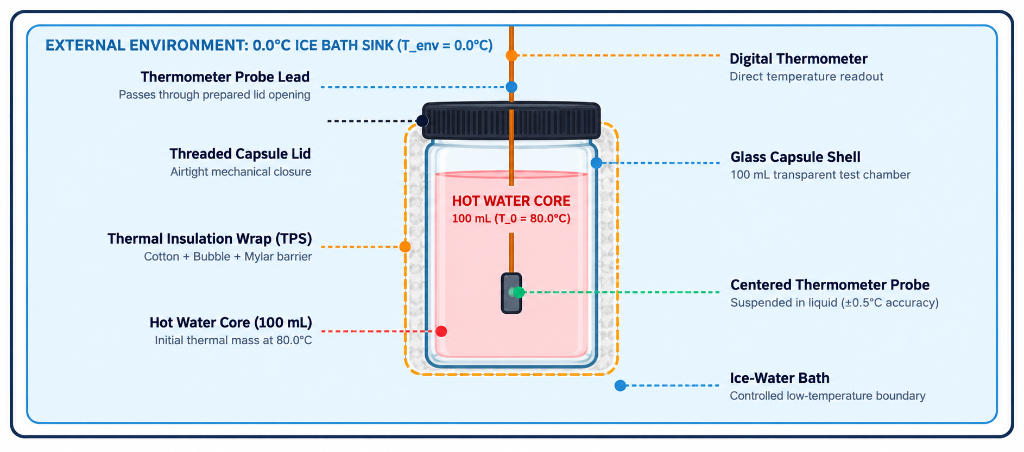
\includegraphics[width=0.98\linewidth]{assets/hardware-schematic.png}\par\vspace{2pt}{\footnotesize Image B. Capsule arrangement showing the warm-water core, centred probe, insulation wrap, and ice-water boundary.}\end{center}

\begin{center}\footnotesize
\setlength{\tabcolsep}{2.5pt}
\renewcommand{\arraystretch}{1.14}
\begin{tabular}{>{\raggedright\arraybackslash}p{0.25\columnwidth}>{\raggedright\arraybackslash}p{0.31\columnwidth}>{\raggedright\arraybackslash}p{0.34\columnwidth}}
\toprule
\textbf{Condition} & \textbf{Construction} & \textbf{Purpose} \\
\midrule
Bare control & Jar with no added insulation & Reference heat-loss path \\
Bubble wrap & Two even layers with cells uncrushed & Trapped-air layer \\
Mylar only & One reflective layer, neck closed & Reflective layer by itself \\
Full MLI & Cotton, bubble wrap, outer Mylar & Combined mechanisms \\
\bottomrule
\end{tabular}
\end{center}

\subsection*{3.2 Construction controls}

Small assembly differences changed the response during development. A probe touching the glass did not represent the bulk water. Tight tape flattened bubble cells. A loose opening around the probe created a direct heat-loss path and could let bath water enter. The team therefore treated probe position, layer compression, closure, and immersion depth as controlled variables.

\begin{itemize}[leftmargin=*,nosep]

\item Use jars with the same diameter, wall thickness, and fill height.

\item Cut insulation pieces to the same nominal size for repeated trials.

\item Secure each layer only tightly enough to stop movement.

\item Keep the jar neck and probe opening as consistent as possible.

\item Record any wetting, gap, leak, or probe movement with the run data.

\end{itemize}

\begin{center}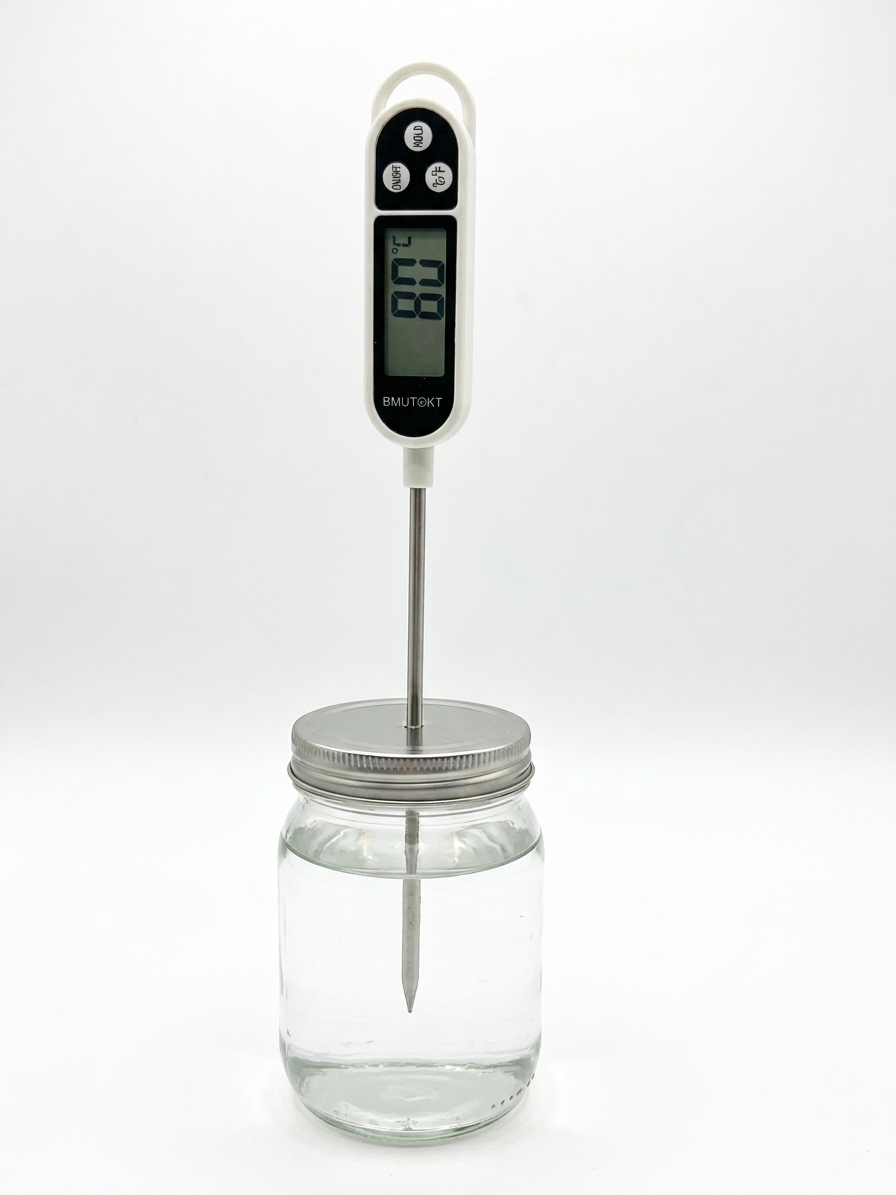
\includegraphics[width=0.53\linewidth]{assets/barecapsule.jpeg}\par\vspace{2pt}{\footnotesize Image C. Bare control capsule with the probe centred through the lid.}\end{center}

\subsection*{3.3 Full multilayer package}

The full package is built from the core outward: cotton next to the jar, two layers of bubble wrap around the cotton, and Mylar on the outside. The order was chosen so the soft inner layer follows the jar, the bubble layer provides trapped air, and the reflective sheet forms the outer surface. This arrangement is a classroom analogue only. Real spacecraft multilayer insulation uses carefully controlled low-emittance films, spacers, vacuum conditions, and qualification tests.

\begin{center}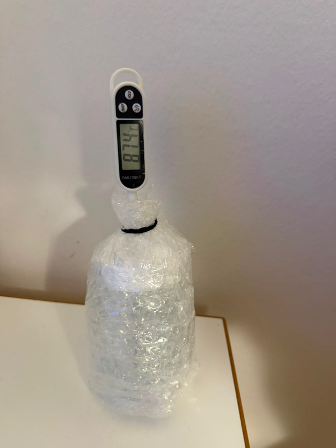
\includegraphics[width=0.43\linewidth]{assets/bubblewrap-only.png}\par\vspace{2pt}{\footnotesize Image D. Bubble-wrap test article with two uncrushed layers and a closed probe opening.}\end{center}

\begin{center}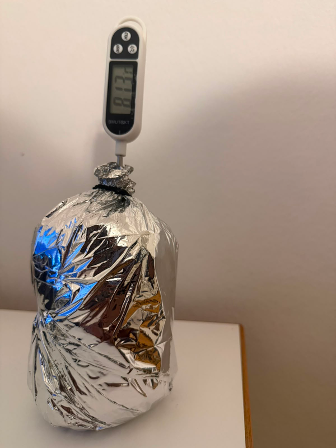
\includegraphics[width=0.43\linewidth]{assets/full-mli.png}\par\vspace{2pt}{\footnotesize Image E. Completed multilayer test article with the external reflective layer and digital probe.}\end{center}

\subsection*{3.4 Integration with the learning kit}

The hardware labels match the configuration names in Mission Control. This prevents a group from choosing one model coefficient while testing another construction. The same four names appear in the manuals, worksheet, result table, and assessment questions.

\section*{4 Experimental Method and Safety}

\subsection*{4.1 Controlled procedure}

\begin{enumerate}[leftmargin=*,nosep]

\item Prepare a stable dry work area. Keep laptops and displays away from the bath.

\item Build the assigned insulation and check the jar with cool water.

\item Prepare the ice-water bath and record its actual temperature.

\item Add 100 mL of water near 80 $^\circ$C and record the actual starting temperature.

\item Centre the probe, close the neck, immerse the jar to the agreed depth, and start the timer.

\item Record the core temperature at t = 0 and once per minute through t = 15 min.

\item Enter the readings without smoothing them. Calculate drop, residuals, MAE, and an effective k.

\item Compare conditions and list the factors that limit the conclusion.

\end{enumerate}

\subsection*{4.2 Fair-test criteria}

Every condition should use the same jar geometry, water volume, probe depth, immersion depth, bath location, and timing method. The bath temperature must be measured rather than assumed. If a reading is late, the actual time should be recorded. A complete run contains 16 ordered time-temperature pairs or a written reason for each missing point.

\subsection*{4.3 Safety precautions and risk assessment}

Risks were assessed qualitatively from the likelihood and consequence of each hazard after controls were applied. The test must stop if a jar cracks, the bath becomes unstable, water reaches an electrical connector, or a significant leak occurs. Hot water is handled only by an adult or trained supervisor, and the work area remains dry and unobstructed.

\begin{center}\footnotesize
\setlength{\tabcolsep}{2.5pt}
\renewcommand{\arraystretch}{1.14}
\begin{tabular}{>{\raggedright\arraybackslash}p{0.18\columnwidth}>{\raggedright\arraybackslash}p{0.20\columnwidth}>{\raggedright\arraybackslash}p{0.36\columnwidth}>{\centering\arraybackslash}p{0.12\columnwidth}}
\toprule
\textbf{Hazard} & \textbf{Main risk} & \textbf{Required control} & \textbf{Residual} \\
\midrule
Hot water & Burn & Supervised pouring; gloves or tongs & Low \\
Glass jar & Cuts or spill & Inspect before use; stable container & Low \\
Water and electronics & Shock or damage & Keep laptops, plugs, and displays dry & Low \\
Unstable bath or leak & Scald or flooding & Stop test; isolate and clean area & Low \\
Wet floor & Slip & Use towels and remove spills immediately & Low \\
\bottomrule
\end{tabular}
\end{center}

\subsection*{4.4 Data quality}

The original readings were retained, including the unexpected Mylar-only curve. The purpose of the model is to support a comparison, not to force a match. Repeating each configuration at least three times and randomising the run order would improve the evidence. Future trials should also record water mass, bath temperature, probe depth, immersion depth, and construction notes for every run.

\section*{5 Software and Data Workflow}

\subsection*{5.1 Architecture}

Mission Control is a browser-based single-page application built with HTML, CSS, and JavaScript. Chart.js draws prediction and telemetry curves, while KaTeX renders the mathematical notation. Local browser storage keeps the selected model, generated prediction, measurements, quiz state, and fallback leaderboard results. The core laboratory runs without a native installation, Bluetooth link, or device driver. The current project also supports an optional Supabase connection for a shared classroom quiz leaderboard; when it is not configured or cannot be reached, the leaderboard falls back to local storage.

\subsection*{5.2 Workflow}

\begin{center}\footnotesize
\setlength{\tabcolsep}{2.5pt}
\renewcommand{\arraystretch}{1.14}
\begin{tabular}{>{\raggedright\arraybackslash}p{0.25\columnwidth}>{\raggedright\arraybackslash}p{0.31\columnwidth}>{\raggedright\arraybackslash}p{0.34\columnwidth}}
\toprule
\textbf{Stage} & \textbf{Website action} & \textbf{Student action} \\
\midrule
Prediction & Calculates T(t) from T0, Tenv, k, and time & Choose a condition and record assumptions \\
Measurement & Provides timer and 16-point log & Read and enter one value per minute \\
Comparison & Overlays measured and predicted curves & Inspect curve shape and residuals \\
Evaluation & Calculates MAE and feedback score & Explain the disagreement physically \\
Assessment & Runs a timed ten-question challenge & Review answers and compare team score \\
\bottomrule
\end{tabular}
\end{center}

\subsection*{5.3 Graphing choices}

The prediction and telemetry use the same time axis and configuration colours. Axes include units, and the plotted interval matches the 15-minute procedure. The data table keeps the measured value separate from the predicted value. This makes it clear which numbers came from the physical test and which came from the model.

\begin{center}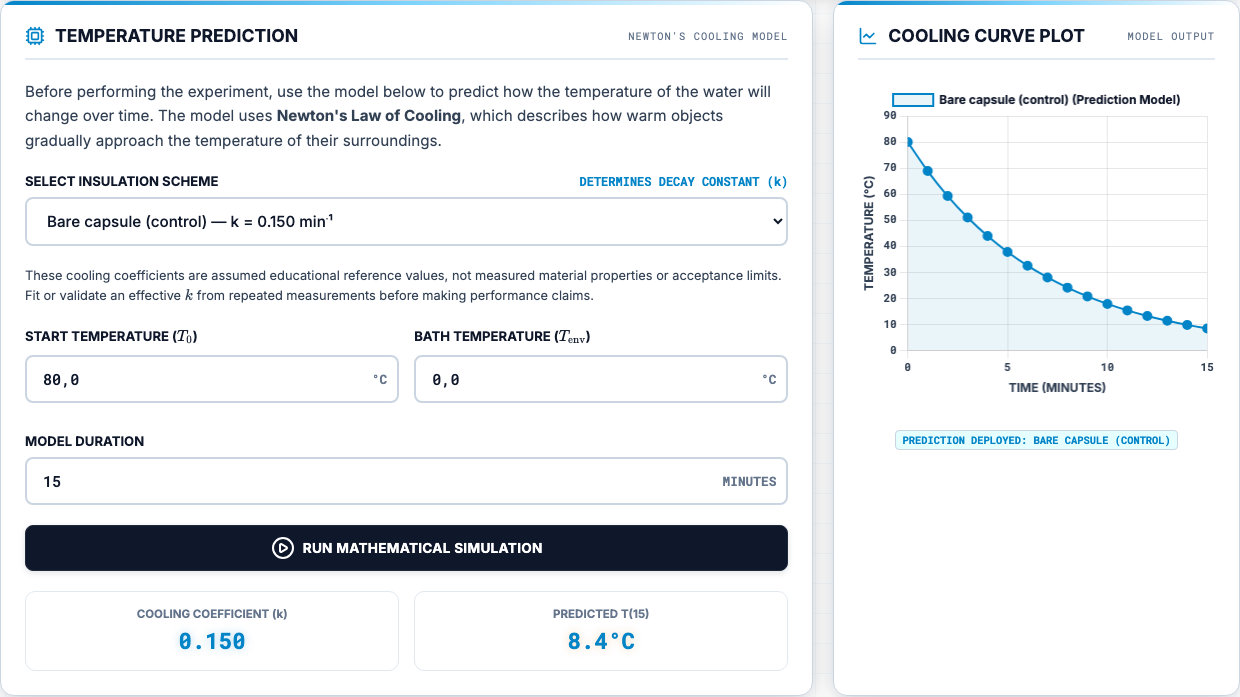
\includegraphics[width=0.98\linewidth]{assets/predicted-curve.png}\par\vspace{2pt}{\footnotesize Image F. Current Mission Control prediction interface and 15-minute cooling curve.}\end{center}

The residual at each time is the measured value minus the model value. The analysis uses mean absolute error as a simple summary:

\begin{equation}\mathrm{MAE}=\frac{1}{n}\sum_{i=1}^{n}|T_{meas,i}-T_{model,i}|.\end{equation}

\subsection*{5.4 Reliability and limitations}

The site is easy to publish with GitHub Pages and can be opened from a local web server. The current build still loads several browser libraries and fonts from public content-delivery networks, so complete offline use requires those dependencies to be bundled locally. The optional shared leaderboard needs the supplied Supabase configuration and database setup; otherwise the application clearly reports local mode. CSV export and structured run metadata remain useful future additions. The dashboard score is classroom feedback, not a formal statistical validation result.

\section*{6 Experimental Results}

\subsection*{6.1 Recorded endpoints}

The worked dataset contains 16 readings for each condition. The endpoint summary is shown below. Because starting temperatures were not identical, final temperature alone is not enough for a fair comparison; the temperature drop and full curve are more useful.

\begin{center}\footnotesize
\setlength{\tabcolsep}{2.5pt}
\renewcommand{\arraystretch}{1.14}
\begin{tabular}{>{\raggedright\arraybackslash}p{0.22\columnwidth}cccc}
\toprule
\textbf{Condition} & \textbf{T0} & \textbf{T15} & \textbf{Drop} & \textbf{Dashboard score} \\
\midrule
Full MLI & 77.6 $^\circ$C & 62.7 $^\circ$C & 14.9 $^\circ$C & 93\% \\
Bubble wrap & 82.6 $^\circ$C & 52.6 $^\circ$C & 30.0 $^\circ$C & 83\% \\
Bare control & 80.1 $^\circ$C & 35.2 $^\circ$C & 44.9 $^\circ$C & 94\% \\
Mylar only & 80.5 $^\circ$C & 33.3 $^\circ$C & 47.2 $^\circ$C & 3\% \\
\bottomrule
\end{tabular}
\end{center}

\subsection*{6.2 Main result}

The full multilayer package had the smallest 15-minute temperature drop and therefore retained the most heat in this run. Bubble wrap ranked second. The bare control and Mylar-only condition cooled much faster. The Mylar-only result does not show that reflective insulation is generally ineffective. It shows that the selected reference coefficient and the physical water-bath construction did not agree for that run.

\subsection*{6.3 Representative telemetry}

\begin{center}\footnotesize
\setlength{\tabcolsep}{2.5pt}
\renewcommand{\arraystretch}{1.14}
\begin{tabular}{>{\raggedright\arraybackslash}p{0.22\columnwidth}cccc}
\toprule
\textbf{Time} & \textbf{Full MLI} & \textbf{Bubble} & \textbf{Mylar} & \textbf{Bare} \\
\midrule
0 min & 77.6 & 82.6 & 80.5 & 80.1 \\
3 min & 75.6 & 72.5 & 55.8 & 59.9 \\
6 min & 73.9 & 65.6 & 44.9 & 47.1 \\
9 min & 70.6 & 60.6 & 38.9 & 40.9 \\
12 min & 67.4 & 56.1 & 35.5 & 37.3 \\
15 min & 62.7 & 52.6 & 33.3 & 35.2 \\
\bottomrule
\end{tabular}
\end{center}

\subsection*{6.4 Fitted cooling constant}

A point estimate of k can be calculated when T(t), T0, and Tenv are known:

\begin{equation}k=-\frac{1}{t}\ln\left(\frac{T(t)-T_{env}}{T_0-T_{env}}\right).\end{equation}

A fit using all usable points is better than a one-point estimate because it uses the curve shape and reduces the influence of one reading. Repeated trials are still needed before reporting material rankings as stable results.

\section*{7 Analysis and Model Limitations}

\subsection*{7.1 Comparison with the model}

The full multilayer package and bare control followed their selected reference curves more closely than the Mylar-only case. The model is useful because it gives the class a common baseline, but k is an effective system value. It changes when the jar, fill, bath, probe, closure, or layer contact changes. A coefficient chosen for one setup should not be presented as a fixed property of a material.

\subsection*{7.2 Likely error sources}

\begin{center}\footnotesize
\setlength{\tabcolsep}{2.5pt}
\renewcommand{\arraystretch}{1.14}
\begin{tabular}{>{\raggedright\arraybackslash}p{0.25\columnwidth}>{\raggedright\arraybackslash}p{0.31\columnwidth}>{\raggedright\arraybackslash}p{0.34\columnwidth}}
\toprule
\textbf{Source} & \textbf{Effect on result} & \textbf{Control} \\
\midrule
Probe touches glass & Biased core reading & Centre probe with a guide \\
Bath warms & Changing boundary & Measure before and during run \\
Different start temperatures & Unfair final-temperature ranking & Use drop, theta, or fitted k \\
Compressed layers & Higher solid conduction & Use repeatable light fastening \\
Water reaches wrap & Extra conductive path & Improve closure and log wetting \\
Timing delay & Shifted data point & Record actual timestamp \\
\bottomrule
\end{tabular}
\end{center}

\subsection*{7.3 Limits of the analogy}

A spacesuit operates in vacuum outside the garment, where there is no external air convection. The classroom jar is surrounded by water, so convection and conduction are strong. Real spacesuits also use an active liquid-cooling and ventilation garment. The activity therefore teaches the method of thermal testing and model checking; it does not reproduce the full physics or certify the materials.

\subsection*{7.4 Confidence in the result}

The recorded ordering is valid as a description of the worked runs: full MLI, bubble wrap, bare control, then Mylar-only by 15-minute temperature drop. Confidence in a general ranking is limited because the available dataset contains one series per condition and incomplete metadata for some construction details. The available evidence does not support a claim that the same ordering will always occur until repeated trials show the variation.

\subsection*{7.5 Changes for the next campaign}

\begin{itemize}[leftmargin=*,nosep]

\item Run at least three repeats per condition and randomise the order.

\item Use a simple probe-position jig and a fixed immersion-depth mark.

\item Record bath temperature at the start and end of every run.

\item Weigh the water instead of relying only on nominal volume.

\item Store construction notes and export all telemetry as CSV.

\end{itemize}

\section*{8 Educational Delivery and Feasibility}

\subsection*{8.1 Classroom sequence}

The lesson starts with a short briefing on heat transfer and the limits of the spacesuit analogy. Groups then predict which condition will retain the most heat, assemble or inspect their test article, run the 15-minute measurement, and compare the recorded curve with the model. The final discussion asks students to defend a ranking and explain at least one source of disagreement.

\subsection*{8.2 Supporting materials}

The current project includes the Mission Control website, student manual, teacher manual and marking guide, task sheet, printable flashcards, illustrated procedure, leaderboard setup guide, and final presentation material. The learning materials use one aligned ten-question framework: written-response questions in the printable set, multiple-choice questions online, and complete solution guidance for students and instructors. The analysis usesd the same configuration names, variables, test duration, and core volume throughout.

\subsection*{8.3 Assessment}

\begin{center}\footnotesize
\setlength{\tabcolsep}{2.5pt}
\renewcommand{\arraystretch}{1.14}
\begin{tabular}{>{\raggedright\arraybackslash}p{0.31\columnwidth}>{\raggedright\arraybackslash}p{0.61\columnwidth}}
\toprule
\textbf{Evidence} & \textbf{What it checks} \\
\midrule
Prediction & Reasoning from heat-transfer mechanisms \\
Raw data table & Careful measurement and units \\
Model comparison & Use of k, residuals, and MAE \\
Evaluation paragraph & Limits, uncertainty, and fair testing \\
Open response & Explanation in the student's own words \\
\bottomrule
\end{tabular}
\end{center}

\subsection*{8.4 Practical feasibility}

The equipment is reusable, and the core laboratory does not require a paid account. Shared multi-device leaderboard synchronisation is optional and depends on a configured Supabase project; local scoring remains available without it. The item estimate is EUR 11 for jars and cable glands, EUR 16 for four digital probe thermometers, EUR 8 for insulation materials, and EUR 5 for the test tub. The EUR 40 total remains a planning value until checked against final receipts.

\begin{center}\includegraphics[width=0.92\linewidth]{assets/budget\_items.png}\par\vspace{2pt}{\footnotesize Budget graph. Item-level planning estimate: EUR 40 total, below the EUR 50 course target.}\end{center}

\subsection*{8.5 Handover}

A teacher should receive the full kit, printed safety checklist, spare insulation, towels, and a local copy of the website. The handover notes should state the measured jar volume, probe type, reference coefficients, and known limits. This information is more useful than a polished demonstration alone because it lets another class repeat the test and compare results.

\section*{9 Conclusions, Responsibilities, and References}

\subsection*{9.1 Conclusion}

The team developed a complete classroom engineering activity that connects a physical thermal test with a simple mathematical model. The full multilayer package retained the most heat in the worked data, while the Mylar-only result showed the importance of boundary conditions and construction. The strongest part of the project is the full workflow: students make a prediction, control a test, keep raw data, compare the result with a model, and explain the mismatch.

\subsection*{9.2 Final recommendations}

\begin{itemize}[leftmargin=*,nosep]

\item Repeat all four conditions and report the variation, not only one curve.

\item Bundle Chart.js and KaTeX locally for offline use.

\item Add CSV export, run identifiers, and metadata fields.

\item Use a probe guide and fixed immersion mark.

\item Verify the final cost from current supplier quotes.

\item Keep the vacuum-versus-water-bath limitation in every student briefing.

\end{itemize}

\subsection*{9.3 Project deliverables}

The submitted engineering package contains the website, classroom documentation, assessment material, experimental procedure, and presentation resources listed below.

\begin{center}\footnotesize
\setlength{\tabcolsep}{2.5pt}
\renewcommand{\arraystretch}{1.14}
\begin{tabular}{>{\raggedright\arraybackslash}p{0.31\columnwidth}>{\raggedright\arraybackslash}p{0.61\columnwidth}}
\toprule
\textbf{Deliverable} & \textbf{Purpose and report connection} \\
\midrule
Mission Control website & Prediction, telemetry, model comparison, quiz, and leaderboard \\
Student manual & Student-facing theory, construction, procedure, and analysis guidance \\
Teacher manual and marking guide & Preparation, safety, solutions, and assessment criteria \\
Task sheet & Prediction, raw data, calculations, evaluation, and open response \\
Printable flashcards & Ten aligned revision and discussion topics \\
Illustrated procedure & Assembly sequence and experimental controls \\
Final presentation & Team overview, method, findings, and classroom delivery \\
README and setup guides & Deployment, resource links, and optional leaderboard configuration \\
\bottomrule
\end{tabular}
\end{center}

\begin{thebibliography}{00}

\bibitem{b1} NASA, "Spacewalk Spacesuit Basics," Johnson Space Center, accessed 9 Sep. 2026.

\bibitem{b2} NIST, "Water Liquid Phase Heat Capacity," Chemistry WebBook SRD 69, accessed 9 Sep. 2026.

\bibitem{b3} M. M. Finckenor and D. Dooling, Multilayer Insulation Material Guidelines, NASA/TP-1999-209263, 1999.

\bibitem{b4} NASA, Passive Thermal Control Engineering Guidebook, Rev. 4.0, 2023.

\end{thebibliography}

\begingroup\normalsize\setlength{\parskip}{2pt}

\section*{Individual Contribution --- Piyath Vithanage}

\subsection*{Role and completed work}

The current Mission Control application and integration of the final project resources formed the main contribution. The browser workflow connects briefing, assembly, prediction, measurement, study material, and assessment. HTML provides the experiment structure, CSS provides the responsive interface, and JavaScript controls the model, timer, telemetry, quiz, and leaderboard behaviour.

The configuration selector, starting temperature, bath temperature, duration, and cooling constant were connected through a common application state. The 15-minute timer and manual telemetry workflow validate entries, store the active model and data, overlay measured and predicted curves, calculate mean absolute error, and produce a printable telemetry record.

\subsection*{Graphing and analysis}

The graphing workflow allows students to compare measured and predicted temperatures on the same time axis. Configuration names and colours remain consistent across the selector, summary, graph, and result table. Residual and mean absolute error calculations turn the graph into an analysis task instead of using it only as a visual display.

The implementation keeps calculated and measured data as separate series and restores the current session from local browser storage. Defensive checks were added around optional interface elements so that one missing panel would not stop the main simulator. The printed telemetry view records the selected configuration, model settings, chart, measurement count, and error result in a form that can be attached to the student task sheet.

\subsection*{Assessment and final integration}

The assessment work covered the timed ten-question classroom challenge, answer review, scoring, winner presentation, and leaderboard. Results are stored locally by default and can synchronise across devices through the optional Supabase configuration. The student manual, teacher manual, task sheet, flashcards, presentation material, and README were aligned with the current experiment and website.

The final integration work included checking the same question topics across online and printable resources, preserving mathematical notation through KaTeX, and maintaining a usable layout on desktop and mobile screens. Recent repository work also covered the three-page task-sheet layout, quiz progress flow, leaderboard fallback behaviour, and consistent naming across the public project pages.

\subsection*{Reliability and maintainability}

Later repository work included defensive interface checks, resource reorganisation, regenerated printable PDFs, and repeated layout corrections. The website, manuals, worksheets, and presentation were treated as one learning system rather than independent files. A changed experimental setting therefore required corresponding updates to the model controls, theory text, task sheet, teacher solution, and result explanation.

The final application keeps the main activity usable when optional services fail. The thermal model and telemetry remain local to the browser. The competitive leaderboard reports its mode and falls back to saved local scores when the shared connection is unavailable. This separation reduces the risk that a network problem stops the laboratory. It also makes the optional database feature easier for another developer or teacher to configure later.

\endgroup

\begingroup\normalsize\setlength{\parskip}{2pt}

\section*{Individual Contribution --- Elio Krollpfeiffer}

\subsection*{Early website and interface development}

The work focused on early development of the SPHERE website and the learning materials that established the project structure. Repository history records 78 commits from the associated development account. Most changes affected index.html, with additional work in styles.css, the student manual, the teacher manual, and project images.

The first versions of the browser interface were developed and revised to organise the main content sections and establish the visual and instructional flow used by the later Mission Control application. This work gave the project a usable web base before telemetry, assessment, and leaderboard integration.

The early interface revisions brought together the project introduction, heat-transfer content, experiment instructions, and supporting visuals in one location. Repeated changes to the main page show an iterative development process rather than a single upload. The structure established a clear path from project context to theory and practical activity, which remained the basis of the final site.

\subsection*{Student and teacher documentation}

Repeated work on the student and teacher manuals established the experiment purpose, task sequence, and information needed while using the website. The teacher material supported lesson preparation and classroom delivery, while revised media assets supported the early interface and documentation.

The documentation contribution was important because the experiment depends on consistent instructions. The manuals needed to explain what students should build, what teachers should prepare, and how the physical activity related to the website. The early revisions supplied this instructional foundation and gave later versions a source that could be refined and aligned with the final settings.

\subsection*{Content architecture and revision}

The early website work also established the relationship between navigation, explanatory text, experiment instructions, and visual material. Keeping these elements in one browser page reduced the number of separate files that students had to manage during the lesson. It also created clear locations for later prediction, telemetry, study, and assessment panels.

Repeated document and interface revisions improved the sequence, terminology, and presentation. The manuals and web interface share one instructional structure, while the final package uses the current experimental settings and expanded application functions.

\endgroup

\begingroup\normalsize\setlength{\parskip}{2pt}

\section*{Individual Contribution --- Dilan Fernando}

\subsection*{Role and completed work}

The main technical responsibility covered the thermodynamic definition of the experiment and interpretation of the physical results. The lumped Newtonian cooling model gives students a manageable equation while retaining the relationship between thermal mass, environmental temperature, and cooling rate. The effective system coefficient k is expressed in min$^{-1}$ and remains separate from material thermal conductivity.

The final test conditions use a 100 mL water core, a starting temperature near 80 $^\circ$C, a measured ice-water bath, and readings every minute for 15 minutes. These settings were connected to the apparatus and student procedure so the model and physical experiment refer to the same system.

The thermal formulation also separated the effective cooling constant from material conductivity. This distinction prevented the website values from being presented as fixed properties of cotton, bubble wrap, or reflective film. The selected coefficients were treated as educational reference values for complete configurations and as quantities that should be tested against measured curves.

\subsection*{Experiment and analysis}

The four-condition comparison was planned and analysed using temperature drop, residuals, mean absolute error, and the fitted cooling constant. The unexpected Mylar-only curve was retained as evidence of a model or construction mismatch. Likely influences included probe position, closure, wetting, layer compression, bath temperature, and unequal starting temperatures.

The analysis retained the original measurement series rather than smoothing points to improve agreement. This decision preserved the evidence needed to discuss uncertainty. It also supported the recommendation to repeat every condition, randomise the test order, measure the actual bath temperature, and record construction details with each run.

\subsection*{Safety, documentation, and integration}

Safety controls were developed for hot water, glass, spills, and electronics. Terminology and sequence were aligned across the student manual, teacher manual, task sheet, procedure, website content, and report, together with the remaining technical writing and project integration.

The technical integration checked that the physical settings, equations, result interpretation, and safety limits did not conflict across documents. This included the 100 mL fill, measured environmental boundary, 15-minute interval, four named configurations, and the limitation that a water bath does not reproduce vacuum heat transfer.

\subsection*{Engineering judgement}

The reporting method uses temperature drop, normalised temperature above the boundary, residuals, mean absolute error, and an effective fitted constant because each measure answers a different question. Using several measures prevents final temperature alone from hiding unequal starting conditions and separates the observed ranking from the strength of the general conclusion.

The thermodynamic work provided the acceptance limits for later software and documentation changes. Any interface revision had to retain the correct units, environmental boundary, time base, and meaning of the coefficient. Any educational revision had to preserve the distinction between spacecraft thermal control and the conductive-convective water-bath demonstration. These checks maintained technical consistency while the presentation of the project changed.

\subsection*{Model behaviour and uncertainty}

The model implementation was checked dimensionally and against limiting behaviour. At the start of a run the calculated curve must equal the entered initial temperature, and over time it must approach the measured bath temperature without crossing it. A larger effective cooling constant must produce a steeper curve under otherwise identical conditions. These checks provided a direct way to verify changes in the browser calculation.

The uncertainty review distinguished measurement repeatability from model adequacy. Probe resolution, reading time, water volume, and bath drift affect the observations, while the lumped-temperature assumption and constant boundary affect the reference curve. Reporting both groups prevents a low dashboard error from being interpreted as proof that the physical model is complete.

\endgroup

\begingroup\normalsize\setlength{\parskip}{2pt}

\section*{Individual Contribution --- Nuhansee Migelhewage}

\subsection*{Principles and theory}

The main contribution covered development and explanation of the scientific principles behind the activity. The theory addresses conduction, convection, radiation, thermal capacity, and transient cooling at the appropriate student level. It connects the classroom water-bath system to the spacesuit context while retaining the important limitation that the experiment does not reproduce heat transfer in vacuum.

The layered insulation system was interpreted by mechanism. Cotton and bubble wrap mainly reduce conductive and convective paths in the classroom setup, while the reflective layer addresses radiative exchange when a suitable gap is present. This explanation supports the prediction task and discussion of why Mylar alone can perform poorly in a water bath.

The theory contribution also covered thermal capacity and the meaning of the effective cooling constant. The water mass stores sensible energy, while the fitted constant represents the response of the complete core, container, insulation, and boundary. Presenting these ideas separately helped students avoid treating the reference coefficient as a material property.

\subsection*{Experimental setup}

Preparation and checking of the physical experiment covered the glass water core, probe position, insulation layers, ice-water bath, and measurement sequence. Fair-test controls included equal water volume, comparable jars, repeatable probe depth, consistent immersion depth, and one-minute sampling so configuration differences could be discussed as engineering results rather than setup differences.

The setup work included checking the layer order for the complete package: cotton next to the jar, bubble wrap as the trapped-air layer, and reflective film on the outside. Particular attention was given to avoiding compressed bubble cells, maintaining a repeatable neck closure, and keeping the probe centred rather than touching the glass wall.

\subsection*{Safety and classroom preparation}

Practical preparation addressed hot-water handling, stable bath placement, leak checks, dry thermometer displays, and separation of electronics from water. These controls linked the theory to a setup that could be demonstrated and repeated in a supervised lesson.

Classroom preparation also required a clear sequence for measuring the bath temperature, adding the warm water, starting the timer, and recording the first reading. Connecting this sequence to the theoretical variables made it easier to explain why each control mattered and how a setup error would affect the curve.

\subsection*{Theory to practice connection}

The mathematical model was connected with the physical observations. A steep curve indicates rapid approach to the boundary temperature, while a shallow curve indicates greater heat retention in the tested system. Relating curve shape to probe placement, water volume, insulation contact, and bath condition gives students a practical way to discuss differences between measured and predicted values.

The setup and theory work also supported the fair-test requirements used throughout the materials. Each group needs a comparable core, a known starting condition, the same sampling interval, and a recorded environmental temperature. When these controls cannot be held exactly, the deviation must be written down and included in the evaluation. This approach turns the practical activity into an engineering investigation rather than a simple demonstration.

\subsection*{Setup preparation and learning resources}

A pre-run inspection sequence was developed around the setup contribution. The jar is checked for damage, the probe is checked at room temperature, the layer order and closure are inspected, and the bath position is confirmed before hot water is introduced. This sequence reduces avoidable setup variation and gives the supervising teacher a clear stop point when a component is unsafe or inconsistent.

The same setup logic was carried into the student manual, teacher manual, task sheet, illustrated procedure, and flashcards. The student-facing resources describe what must be observed and recorded, while the teacher material explains preparation, safety, and the reason for each control. This alignment helps the physical lesson follow the same sequence as the model and telemetry interface.

The assessment material draws directly on the practical activity. Questions cover conduction, convection, radiation, effective cooling rate, fair testing, and the limitations of the spacesuit analogy. The assessment therefore tests interpretation of the experiment instead of recall of unrelated definitions.

\endgroup

\end{document}